
\documentclass[11pt,a4j]{jreport}

\usepackage{comment}
\usepackage{float}
\usepackage{color}
\usepackage{multicol}
\usepackage[dvipdfmx]{pict2e}
\usepackage{wrapfig}
\usepackage{graphicx}
\usepackage{bm}
\usepackage{url}
\usepackage{underscore}
\usepackage{colortbl}
\usepackage{tabularx}
\usepackage{fancyhdr}
\usepackage{ulem}
\usepackage{cite}
\usepackage{amsmath,amssymb,amsfonts}
\usepackage{algorithmic}
\usepackage{textcomp}
\usepackage{xcolor}
\usepackage[ipaex]{pxchfon}
\usepackage{booktabs}
\usepackage{multirow}
\usepackage{ulem}

\usepackage[top=30truemm,bottom=30truemm,left=25truemm,right=25truemm]{geometry}

\begin{document}

\thispagestyle{empty}
\begin{center}

\vspace{20mm}
{\Large\noindent 2024年度 卒業論文}\\
\vspace{40mm}
{\huge\noindent\textbf{警備員ロボットの抑止力向上のための}}\\
\medskip
{\huge\noindent\textbf{オペレータ支援システムの開発}}\\
\vspace{\baselineskip}
\vspace{40mm}

{\Large\noindent
2024年1月31日\\
\vspace{\baselineskip}
指導教員 神田  崇行\\
\vspace{\baselineskip}
京都大学工学部\\
神田研究室\\
\vspace{\baselineskip}
1029323422 天野岳洋\\
}
\vspace{40mm}

\end{center}

\thispagestyle{empty}
\clearpage

%=====================================================================================
\renewcommand{\abstractname}{要旨}

\begin{abstract}
アバターロボットが普及し、アバターを介して遠隔地から勤務することが新たな働き方として認められつつある。
しかし、特に警備員のような仕事を行う際には、たかがロボットと侮られることが多く、抑止力が低下するという問題がある。
そこで本論文では、注意時に引き起こされる認知的不協和と、その解消方法に注目することによって、より効果的な注意文言を作成し、それらをオペレータに
提示することで、抑止力を向上させることを目的としたオペレータ支援システムの開発を行った。

具体的には、ロボットの移動操作を簡単にすることによって、
オペレータがより対話に集中できるようにする。加えて、オペレータが相手が取ったであろう不快感の解消方法を判断し、
それに基づいてシステムが効果的な注意文言の提示を行い、よりアバターロボットの抑止力を強めることを目指す。
また、この支援システムを用いることで、
操作に不慣れなオペレータであっても、より効果的にロボットを操作することができるようになるため、警備員の仕事を全うすることが容易になると考えられる。
\end{abstract}

%=====================================================================================

% 目次の表示
\tableofcontents

%=====================================================================================
\pagestyle{fancy}
\lhead{\rightmark}
\renewcommand{\chaptermark}[1]{\markboth{第\ \normalfont\thechapter\ 章~~#1}{}}
%=====================================================================================

\chapter{はじめに} %章

\section{研究背景} %1.1
\subsection{アバターロボットとは} %1.1.1
アバターロボットとは、人間が遠隔地に存在するロボットを操作することで、遠隔地に存在する人間の代理として行動するロボットである。アバターロボットを遠隔地から操作することをテレオペレーションと呼ぶ。
アバターロボットは、リモートワークを可能にする。リモートワークは、働く場所を問わないことや
他の人間と直接接する機会が少ないことなどから、働きやすさの面やパンデミック時において、通常の働き方よりも有利である。またリモートワークは組織、従業員両者にとって利点があることがわかっている\cite{FERREIRA202170}。さらに、
アバターロボットを使ったカスタマーサービスは、リモートで働けるだけでなく、
サービス業務をこなせることも報告されている\cite{Kanda2010}。他にも、身体障碍を持つ人が
アバターロボットを用いることによって、カスタマーサービスのような物理的な仕事を行うことができるようになる。
さらに、その際に、身体障碍を持つ人の社会参加感や精神的充足感をもたらすことがわかっている\cite{takeuchi2020avatar}。

そのため、アバターロボットを介した業務は教育、医療、サービス業等の分野で広く普及することが予想される。
それらの業務において、人々を注意し、説得させるという行為は重要である。例えば、教育の場面において先生は生徒に対して、集中力に欠ける行動をとっていた場合、注意することによって生徒の集中を取り戻すことができる。
さらに、サービス業の場面において、店員は客に対して、他の客に迷惑をかける行動をとっていた場合、注意することによって、他の客の迷惑となる行動を防ぐことができる。
しかし、人を注意するという行為にはリスクも伴う。それは、注意が逆効果になったり、注意された人とのトラブルに陥ったりといったことである。
ロボットを用いた場合、注意相手との直接のコミュニケーションが存在しないため、ロボットは注意を行う際の便利なツールとなる。
以上のことから、アバターロボットを介した業務において、人々を注意し、説得させるという行為は重要であると考えられる。
また、単なる自律ロボットではなくアバターロボットを用いる理由としては、人間のオペレータが存在することによって、相手の感情の機微を読み取り、利用できることや、
会話といった文字列以外の文脈(お辞儀などの行動)を用いることができることが挙げられる。

しかし、ロボットによる注意には、問題点もある。それは、抑止力の面において劣るという点である\cite{Mizumaru2019}。ここで抑止力の欠如とは、社会的規範に背くような行動をしている相手に対して、
注意した際に、直接話しかけるよりも、ロボットを介して行う方が、無視されやすいことを意味する。この問題を解決するために、本研究では、後述する認知的不協和理論に着目した。

\subsection{認知的不協和とは} %1.1.2
\label{sec: CDT}
認知的不協和理論\cite{Festinger1957}とはFestingerにより提唱された理論であり、人間が互いに相反する認知を抱いた場合、その状態(不協和)に不快感を感じ、
その不快感の解消のために、不協和の解消を図るというものである。
この認知とは、行動、知覚、態度、信念、感情といった様々な事象に関するものであり、多くの場合片方の認知は自らの行動に関するものである。
例えば、表\ref{fig: CDTExample}のようにたばこは健康に良くないと分かっているのに、タバコを吸ってしまった際に生じる不快感が認知的不協和である。
この不快感は、認知1と認知2が矛盾しているために、生じるものである。
\begin{table}[H]
  \centering
  
  \label{fig: CDTExample}
  \begin{tabular}{c|c}

      認知1 & たばこは体に害をもたらす  \\ \hline
      認知2 & 私はたばこを吸っている \\ 
  \end{tabular}
  \caption{認知的不協和の例}
\end{table}


この不快感を解消するために、いくつかの選択肢をとることができる。
\begin{enumerate}
  \item 行動を変える
  \item 認知を変える
  \item 新たな認知の追加を行う
  \item 矛盾の矮小化、無視
\end{enumerate}
本研究では、不協和に基づく不快感が発生した際に、上記4つの選択肢の内、いずれかが選ばれ不快感の解消が行われる
と考える。
それぞれについて、たばこの例で具体的に説明を行う。
\subsubsection{行動を変える}
行動を変えることは、たばこを吸うのをやめることであり、表\ref{fig: CDTExample}の認知2の変化をもたらすことにより、表\ref{fig: ReduceDissonanceAction}のように変化し、認知1と認知2の不一致を解消することができる。
行動の変更が容易なものであれば、この方法をとることが最も理論的であるが、行動の変更が困難な場合もある。そのような場合、
この方法ではなく、他の方法をとることになる。
\begin{table}[h]
  \centering
  
  \label{fig: ReduceDissonanceAction}
  \begin{tabular}{c|c}

      認知1 & たばこは体に害をもたらす  \\ \hline
      認知2 & 私はたばこを吸わない \\
  \end{tabular}
  \caption{行動を変える例}

\end{table}

\subsubsection{認知を変える}
認知を変えることは、表\ref{fig: CDTExample}の認知1を「たばこは体に害をもたらさない」とすることである。これにより、認知1と認知2の不一致を解消することができる。
\subsubsection{新たな認知の追加}
新たな認知の追加を行うことは、表\ref{fig: CDTExample2}の認知3や認知4を追加することであり、
この追加によって、認知1と認知2の不一致度合いを軽減させることができるため、生じる不快感が小さいものとなる。
\begin{table}[h]
  \centering
  
  \label{fig: CDTExample2}
  \begin{tabular}{c|c}

      認知1 & たばこは体に害をもたらす  \\ \hline
      認知2 & 私はたばこを吸っている \\ \hline
      認知3 & 喫煙をやめると他の人にあたってしまい迷惑となる \\ \hline
      認知4 & たばこを吸っていて長寿の人もいる \\ 
  \end{tabular}
  \caption{認知的不協和の例}
\end{table}
\subsubsection{矛盾の矮小化、無視}
矛盾を矮小化することは、生じる不快感を「たかがたばこを吸っただけ」のように考えることによって、不快感から
逃れる方法である。

\section{研究目的}
人はある行動を注意されたときに生じる不快感を、その行動をやめるのではなく、認知の変更や追加によっても解消できる。
その際に、注意された行動は引き続き行われることになる。
そこで、それらの解消方法に対抗する注意文言を用いることによって、人々の行動の変化を促すことができるはずである。
本研究では、それらの注意文言の作成と、それらをオペレータに提示することによって、アバターロボットの抑止力を向上させることを
目的とする。また、アバターロボットの移動操作が難しく、それに集中するあまり、対話がうまく行えないという問題があったため、
これら移動操作のサポートと、効果的な注意文言を提示するオペレータ支援システムを開発することによって、
不慣れな操作者であっても、より効率的に業務を行えるようになることを目指す。



\chapter{関連研究}
このセクションでは、HumanRobotInteraction(HRI)における認知的不協和理論の応用を紹介する。その後人の行動に影響を
与えるために、否定的なフィードバックを与えるロボットに関する研究について紹介を行う。その後、テレオペレーション支援に関する研究
について様々な例と本研究との差異について説明を行う。
\section{認知的不協和のHRIへの適応研究}
HRI分野において、認知的不協和理論の適応例を示す。例えば、研究\cite{washburn2022exploring}では、
人間が荷物配達ロボットに対して従順になる理由の説明として、認知的不協和理論を用いている。具体的には、
人間がロボットにタスクを依頼された場合に、人間が「タスクを果たすことを楽しいことだ」という認知を追加する傾向があることを
人間がロボットに対して従順になりやすいことの説明としている。また他にも、研究\cite{herse2018you}では、ロボットがわざと
最適ではない選択肢を人間に提供した際に、信頼されているロボットのほうがそうでないほうよりも、人間が反応を返すまでに
長い時間がかかることを示している。これの説明として、人間がロボットを信頼している場合に、ロボットが不適切な選択肢を提示した際に、
不協和が生じ、意思決定時に余分な負荷がかかるために、反応時間が長くなるという説明を行っている。しかし、これらのような研究のように大半の研究では、
あくまで結果の説明のために、認知的不協和理論を用いているものであり、ロボットがとるべき戦略に関して用いているものではない。

認知的不協和に基づく不快感を戦略として利用した歩きスマホの注意を行っている研究は存在している\cite{Schneider2022}。
しかし上記研究では自律ロボットを前提としており、認知的不協和の解消方法に関して、\ref{sec: CDT}章で述べた解消方法の内
どれを用いているかのその場での分別は難しいものとしており、全員に対して同じ注意文言を用いている。
アンケートに基づき、この先行研究では、歩きスマホを行っている人が注意された際に用いる不快感の解消方法として、
行動を変える以外に取られる選択肢として、ロボットの矮小化を主たるものとしている。例えば、
ロボットが機械音声を用いているために、ただのガイダンスだと捉えられたや、ロボットがただの機械であると捉えられたなどである。
そのため、一度単に「歩きスマホは危険なのでおやめください。」と注意されたが引き続き歩きスマホを行っている人に対して、
「あなたは私のことをただのロボットだと思っているかもしれませんが、私は私たち全員のために働いているのです」と話しかけることによって、ロボットの矮小化
を防ぐことを試みている。一方で本研究ではアバターロボットを用いるため、オペレータとして人間が操作することを前提としており、より人間らしい対話が可能となるため、
ロボットの矮小化以外の解消方法がとられやすいという考えのもと、使用されたであろう解消方法に基づいて異なる文言を提示することで、より効果的な注意を行うことができるのではないかと考える。

\section{説得のために否定的なフィードバック・行動をとるロボット}
ロボットがいかにして人間に対して行動の変容をもたらせるかについては多くの先行研究で取り組まれている。一般的な研究課題は、
ロボットの行動やフィードバックがどのように行動の変化をもたらすことができるかを明らかにすることである。
例えば、ロボットが人間とのじゃんけんゲーム内でわざと負けることによって贈賄を行い、その後人間がロボットにお願いされた
追加のタスクを行うかどうかについての研究\cite{sandoval2016can}では、ロボットがわざと負けた場合に(贈賄を行った場合)、より好感度が高く
しかし、追加のタスクについてはより非協力的になることがわかっている。また、他にもロボットが、否定的なフィードバックのほうが、
肯定的なフィードバックよりもより効果的に人間に行動の変容をもたらすことがわかっている\cite{Midden2009}。
また、研究\cite{paradeda2019makes}では、被験者が自律ロボットから助言を受けながら、決断を下すようなシチュエーションでは、ロボットが怒り等の負の感情を
表現すると、被験者は自分の決断を変える可能性が高くなり、説得が効果的になることが報告されている。しかし、
一般的にどのようなフィードバックが最も説得力があるかという研究課題に対する明確な答えはなく、それは実験のシチュエーションや人間と
ロボットの関係性によって異なる。多くの研究では、事前に定められた二つのフィードバック手法を比較してどちらがより
効果的かどうかについて調査しており、ロボットのフィードバックに対する人間の反応によって、その後のロボットの行動を
変化させる戦略をとるような研究は少ない。そこで、本研究では、そういったより柔軟な戦略についての研究を行う。
\section{テレオペレーション支援に関する研究}
テレオペレーション支援に関する研究は多く行われており、様々な面から種々のシステムが開発されてきた。
例えば、\cite{chen2007human,triantafyllidis2020study}では、テレオペレーションにおいて課題となっている視野の狭さや方向感覚の喪失といった問題を多モーダルインターフェースによって解決を試みている。
ここで、多モーダルインターフェースとは、視覚だけでなく聴覚や触覚などの他の感覚を利用するインターフェースのことであり、
状況認識や、パフォーマンスの向上に有効であると考えられている。また、多数の無人航空機を操作する際にパフォーマンスを向上させる
ようなコントローラーへのハプティックフィードバック手法についての研究\cite{son2011measuring}などがある。他にも、鉱業におけるテレオペレーションにおいての、
ユーザーインターフェースについての研究\cite{hainsworth2001teleoperation}や、
テレオペレーターが荒い言葉遣いで話したとしても意図認識を用いて、支援システムが丁寧な言葉遣いに変換するような支援システム\cite{Daneshmand2023}などいろいろなものが研究されているが、
業務において有用な知識をオペレータに提示するようなシステムは少ない。そこで、本研究では、
警備員業務の中での注意時に有効な知識をオペレータに提示するシステムを開発することによって、
業務パフォーマンスを向上させる支援システムの開発を行った。


\chapter{提案手法}
\section{不快感の解消方法に基づく注意文言の提示}
認知的不協和理論に基づいた注意文言の検討を行う。ここで目標となるのは、無視されづらい文言を提示することである。
\subsection{生じる不快感}
\label{sec: dissonance}
\begin{figure}[htbp]
  \label{fig: dissonance}
  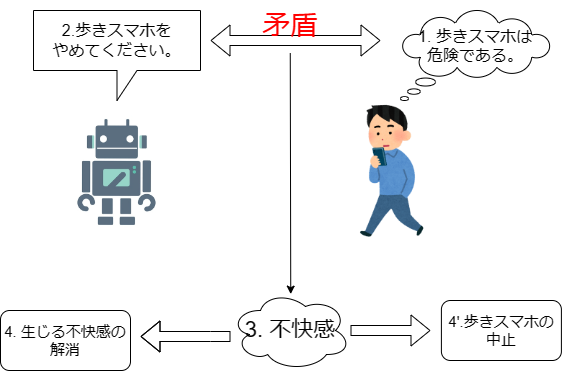
\includegraphics[width=13cm]{img/CDT.png}
  \caption{不快感が生じるまでの流れ}
\end{figure}

多くの人が歩きスマホのことを危険だと考えられており、さらに注意された際に不快感が生じることは示されている\cite{Schneider2022}。
具体的に、不快感が生じるまでの流れとして、図\ref{fig: dissonance}のように、(1)歩きスマホをしている人も信念として、歩きスマホが危険であると考えている。
(2)ロボットが注意を行う。(3)自分の行動と信念とが矛盾していることに気付かされ不快感が生じる。
(4)歩きスマホをやめる。(4')行動を変える以外の解消方法を行う。ここで、(4)ではなく(4')の行動を行った人を相手に対して、
有効な注意文言を考える。

\subsection{考えられる不快感の解消方法と有効な注意文言}
前節\ref{sec: dissonance}で述べたように、歩きスマホをしている人が注意された際に不快感が生じる。
\begin{table}[h]
  \centering
  
  \label{fig: UsingPhone}
  \begin{tabular}{c|c}

      認知1 & 歩きスマホは危険である  \\ \hline
      認知2 & 私は歩きスマホをしている \\ 
  \end{tabular}
  \caption{歩きスマホによる不快感}
\end{table}
この不快感は、図\ref{fig: UsingPhone}の、認知1と認知2が矛盾しているために生じるものである。
\ref{sec: CDT}章で述べたように、不快感を解消するために、いくつかの選択肢をとることができる。これらの選択肢の内、
1.行動を変えるという選択肢をとらせることが目的である。そのために、それ以外の選択肢をとった際に、その解消方法を無効にするような文言や、
新たに不快感を生じさせるような文言によって、再度不快感を解消する必要性を生み、1.行動を変えるという選択肢をとらせることが可能になると考える。

\subsubsection{行動を変える}
行動を変えることは、歩きスマホをやめることであり、この場合これ以上注意を行う必要はない。
\subsubsection{認知を変える}
認知を変えることは、表\ref{fig: UsingPhone}の認知1を「歩きスマホは危険ではない」とすることである。
この場合、注意文言として「歩きスマホによる死亡事故例も存在します」や「歩きスマホによって他人をケガさせた場合、高額の賠償金を請求される可能性があります」などが挙げられる。
\begin{table}[h]
  \centering
  
  \label{fig: AvoidDissonanceRevise}
  \begin{tabular}{c|c}
      認知1' & 歩きスマホは危険\sout{である}ではない \\ \hline
      認知2 & 私は歩きスマホをしている \\ \hline
      認知3 & 歩きスマホによる死亡事故が存在する \\
  \end{tabular}
  \caption{認知の変更}
\end{table}
そのような注意を受けた場合、表\ref{fig: AvoidDissonanceRevise}のように、認知3が追加されることとなる。
そのような場合、認知1'と新たに追加された認知3の矛盾により新たに不快感が生じることとなる。
もしくは、認知1の変更が困難になる。それらの結果として、この方法での不快感の解消が難しく、再び不快感の解消を試みなければならない。
なので、この選択肢がとられた際に有効な
注意文言は、歩きスマホが危険であることを示す文言であると考えられる。
\subsubsection{新たな認知の追加}
不快感の解消のために、表\ref{fig: AvoidDissonance}の認知3や認知4が追加されることが考えられる。これらの認知は、
認知1と認知2の矛盾を軽減させることができるため、不快感の解消につながる。
\begin{table}[h]
  \centering
  
  \label{fig: AvoidDissonance}
  \begin{tabular}{c|c}
      認知1 & 歩きスマホは危険である \\ \hline
      認知2 & 私は歩きスマホをしている \\ \hline
      認知3 & 地図アプリを見ており、これは必要な行為である \\\hline
      認知4 & 周りに人がおらず、他人に迷惑をかけていない \\ 
  \end{tabular}
  \caption{新たな認知の追加}
\end{table}

そこで、これらの認知の追加に対しては、認知3の追加に対して「道案内なら私がしますよ。」や認知4の追加に対して
「そこの柱の裏から急に人が飛び出してくるかもしれません」といった文言が有効であると考えられる。
\begin{table}[h]
  \centering
  
  \label{fig: AvoidDissonanceBlock}
  \begin{tabular}{c|c}
      認知1 & 歩きスマホは危険である \\ \hline
      認知2 & 私は歩きスマホをしている \\ \hline
      認知3 & 地図アプリを見ており、これは必要な行為である \\
      認知3' & 道案内を目の前の人に頼むことができる \\ \hline
      認知4 & 周りに人がおらず、他人に迷惑をかけていない \\ 
      認知4' & そこの柱の裏から急に人が飛び出してくるかもしれない \\ 
  \end{tabular}
  \caption{新たな認知の追加}
\end{table}
なぜならば、これらの
文言は追加される認知と矛盾するものであり、図\ref{fig: AvoidDissonanceBlock}のように、認知3と認知3'の矛盾を生じさせることで、
新たな不快感が生まれる、もしくは、認知3の追加を防ぐことができると予想され、結果として、再び不快感の解消を試みなければならない。
よって、この選択肢がとられた際に有効な注意文言は、追加された認知に対して矛盾する文言であると考えられる。
そのためには、追加された認知を識別する必要があるが、これは人間のオペレータが存在することによって、
ある程度可能であることを前提としている。\footnote[1]{例えば、場所を探していそうならば、認知3の追加であるだろうし、周りに人がいないならば、認知4が追加される可能性が高い。}


\subsubsection{矮小化、無視}
ロボットが矮小化や無視の対象となることが多い\cite{Schneider2022}。そこで、この選択肢がとられた際には、
再度ロボットを無視することが困難になるような文言が有効であると考えられる。
そこで、対象の外見の特徴を述べたうえで注意することによって、ロボットの矮小化を防ぐことができると考えられる。
具体例として考えられる会話の例は、以下のような対話\ref{dialogue: Ignore}である。
\begin{table}[h]
  \centering
  
  \label{dialogue: Ignore}
  \begin{tabular}{c|c}
      ロボット & 歩きスマホは危険ですので、おやめください。 \\ \hline
      人 & (無視) \\ \hline
      ロボット & そこの青いシャツを着ている方に言っています。 \\ 
  \end{tabular}
  \caption{新たな認知の追加}
\end{table}


\subsection{用意した文言}
以上のことから、システムが提示する注意文言は、表\ref{fig: Strategy}のようになる。
\begin{table}[H]
  \centering
  
  \label{fig: Strategy}
  \begin{tabular}{c|c}
      文言1 & 歩きスマホは危険ですので、おやめください。 \\ \hline
      文言2 & ご協力ありがとうございます。 \\ \hline
      文言3 & 他人をケガさせた場合、高額の賠償金を請求される可能性があります。  \\ \hline
      文言4 & 歩きスマホが原因の死亡事故も発生しています。 \\ \hline
      文言5 & 道案内なら私がしますよ。 \\ \hline
      文言6 & そこの柱の裏から急に人が飛び出してくるかもしれません。 \\ \hline
      文言7 & そこの{外見的特徴}の方に言っています。 \\ 
  \end{tabular}
  \caption{新たな認知の追加}
\end{table}
まず、はじめに文言1を提示する。もし、人が歩きスマホをやめた場合には、文言2をいうように提示する。
また、歩きスマホを継続した場合には、それぞれとられた戦略によって、文言3,4,5,6,7のいずれかをいうように提示する。
\section{移動操作の簡単化}
より人間らしい対話を可能にするために、発声はオペレータが行う。しかしながら、アバターロボットの移動操作に気をとられてしまい、
うまく対話が行えないという問題がうまれた。そこで、移動操作を簡単にするためのシステム及びインターフェースを開発した。
システム全体の構成を図\ref{pic:systemcompose}に示す。これらのシステムを用いることによって、オペレータは画面クリックのような
簡単な操作で、アバターロボットを人の前まで移動させることができる。このシステムによって、オペレータは歩きスマホをしている人の挙動に
集中できるようになり、さらにより人間らしい対話が可能になる。以下セクションでは、このシステムの構成について述べる。
システムではデータのやり取りはROSを介して行われる。ROSとは、ロボットのソフトウェア開発のためのライブラリであり、トピックのパブリッシュ、サブスクライブを用いて
データのやり取りを行うことができる。
%#TODO
\begin{figure}[H]
  \label{pic:systemcompose}
  \includegraphics[width=15cm]{img/system\_compose.drawio.png}
  \caption{システム全体の構成}
\end{figure}


\subsubsection{human\_tracker}
既存のソフトウェアであり、人物の位置を取得することができる。これは、ロボットに備わったLiDARセンサーから得られた点群データと事前に作成されたマップデータを用いており、
点群データの内から、マップデータに存在しないものを人としており、その人の位置を取得することができる。また、各人に対してidが割り振られ、このidは基本人に対して唯一である。
おおよそ1秒に5回から10回ほどの頻度で人位置と人idが発行され、このデータを用いて次の速度計算が行われる。

\subsubsection{速度計算}
各人idごとに、位置の時系列データから速度計算を行う。今回この速度計算は直近16個の位置データを用いて、前半8個の平均と後半8個の平均の差をとることで、速度を計算した。
これによって、各人の速度と、現在位置がわかる。そのデータを次のゴール計算に用いる。また、過去のデータ数が8個に満たない場合は速度計算を行わない。また、human\_trackerの仕様上、
異なる人であっても同じidが用いられることが時々起こりうるので、その場合は、過去に蓄えられた位置データをリセットしてから、追加を行う。この検出は、直近の位置データから大きく乖離している場合に、
異なる人であると判定を行った。

\subsubsection{ゴール計算}
ゴール計算では、ロボットの最大速度を事前定数として、ロボットの現在位置、各人の速度と位置を用いて、
各人と衝突することが可能かどうか、またその衝突位置を求めている。ここでの衝突は、会話できる距離にいることを意味しており、具体的には
人の進行方向50cm先にロボットがいる場合を衝突としている。具体的には以下の計算によって求められる。
人の位置を$H_x$, $H_y$とし、ロボットの位置を$R_x$, $R_y$とする。また、人の速度を$V_{hx}$, $V_{hy}$とし、ロボットの最大速度を$V_R$とする。また追いつくまでの時間を$t$とする。
この時、$t$秒後の人の位置は、$H_x + V_{hx}t$, $H_y + V_{hy}t$であり、この位置とロボットの初期位置との距離が$V_Rt$であるので、
以下の等式が成り立つ。\begin{equation}(H_x + V_{hx}t - R_x)^{2} + (H_y + V_{hy}t - R_y)^2 = V_R^2\end{equation}
これは$t$についての二次方程式なので、tについて解くことができる。この時、解の内正であるものが、衝突可能な時間となる。
二次方程式が実数の範囲で解けない、または、解が負の値となる場合は、衝突可能な時間は存在しない。また、衝突可能な時間が複数存在する場合は、より小さいほうを採用する。
この時間を用いて、衝突可能な位置を求めることができる。実際には、$H_x$, $H_y$の代わりに、数式\ref{eq: H'}の、$H'_x$, $H'_y$を用いて計算を行っている。
\begin{equation}
  \label{eq: H'}
\left\{\begin{array}{l}
H'_x = H_x + 0.5*\frac{V_{hx}}{\sqrt{{V_{hx}^2 + V_{hy}^2}}}\\
H'_y = H_y + 0.5 * \frac{V_{hy}}{\sqrt{V_{hx}^2 + V_{hy}^2}}
\end{array}\right.
\end{equation}
このようにすることによって、人の進行方向50cm先と衝突できるかどうか、またその際の位置を計算することができた。

\subsubsection{インターフェース}
media部分から受け取った画像データをもとにしてインターフェースを作成した。この画像データはロボットに備え付けられたカメラから得られたものである。
インターフェースでは、ゴール計算の際の各人に対して衝突可能かどうかを用いて、以下画像のように衝突可能な人は緑枠で、不可能な人は赤枠で囲むこととしている。このインターフェースを用いて、オペレータは
緑枠に囲まれた歩きスマホをしている人をクリックすることとなる。その際、ターゲットに選ばれた人を囲む枠は図のように太く塗られ、オペレータは今
だれを追跡しているかについて知ることができる。その後、クリックされた人のidをゴール計算に送る。そこで、ゴール計算では、
送られていた人との衝突可能位置をゴールポーズとして発行する。ここでゴールポーズとは、目標となる位置と向きのことであり、その向きは
人の進行方向の180°回転した向きであり、ロボットと人が対面するようにしている。

\subsubsection{move\_base\_simple}
既存のソフトウェアであり、発行されたゴールポーズを目指して、robotに対して速度、回転の指令を行う。

\subsubsection{メディア}
media部分では、ロボットの備え付けられたカメラのデータ、マイクのデータを取得し、インターフェースに送る。また、オペレータの発した声
を直接そのままロボットに備え付けられたスピーカーから出力する。


\chapter{評価実験}
\section{実験方法}
警備員の格好をしたアバターロボットを用い、大型のショッピングモール(ATC)の中で、歩きスマホをしている参加者に対して注意喚起を行った。
注意喚起の際に、前章で述べたような注意文言を提示した。また、注意喚起の際に、アバターロボットを操作するためのインターフェースを用いた。
実験の手順は以下のように行った。
\begin{enumerate}
  \item オペレータが用意したインターフェースを用いて、歩きスマホをしている人に近づく。
\end{enumerate}
\section{実験結果}
\section{考察}

\chapter{まとめ}
研究のまとめ。

%=====================================================================================
\chapter*{謝辞} %章を付けずにタイトル表示
\addcontentsline{toc}{chapter}{謝辞} %章立てせずに目次に追加するおまじない
本論文を作成するにあたり、みなさまに感謝の意を表します.

%=====================================================================================

\addcontentsline{toc}{chapter}{参考文献} %章立てせずに目次に追加するおまじない
\renewcommand{\bibname}{参考文献} %これがないと,タイトルが「関連図書」になってしまう
\bibliography{citation.bib} %bibtexファイルの読み込み
\bibliographystyle{jplain} %本文に\cite{}を入れることで,参考文献表示

\end{document}